\chapter{Literature Review and Geometric Models} \label{ch:background}

\section{Introduction}
%not sure what to put here, maybe combine with rbm section
This section details the the basic phenomenon behind rotor blade modulation along with its significance in other applications, and the defining characteristics that allow its use in this application. The second part of this section describes the geometric models for the 2 dimensional case and several 3 dimensional cases. These models will form the basis for verification of the simulations.

\section{Literature Review}
%this is the literature review section on what rbm is and current research in the area
The rotating blades of the helicopter modulate signals that hit the blades by reflecting them. The reflected signal, through the doppler effect, become shifted in frequency in relationship to the velocity of the reflection point \cite{YiminZhang2000}. The rotor blade modulation (RBM) has a complex form and is influenced by several object parameters. These parameters range from the positioning of a signal source to the physical dimensions of the rotor blades. 

The resulting modulated signal has been used in several RADAR applications. First to determine the specific characteristics of a noncooperative helicopter using time frequency analysis in \cite{Bullard1991} that defines a specific signature for physical parameters of a helicopter. The ability to detect a hovering helicopter based on the blade flashes caused by reflected RADAR pulses off the blades is examined in \cite{Misiurewicz1997} where they used information the time domain to determine if a helicopter was hovering. The micro-doppler produced by the RADAR reflection in \cite{Thayaparan2007} is used to determine the rotation rate of both the main and tail rotor blades using the wavelet transform. Other types of aircraft produce modulations on a returned RADAR pulse, one type known as Jet Engine Modulation (JEM) is the product of a RADAR pulse reflecting off the jet engine blades \cite{NavalAirSystemsCommand1999}. The information can similarly be used to quantify physical aspects of the aircraft when present in order to perform classification.

The doppler shifted signal caused by RBM is shown in \cite{F.BarbieroF.VincentT.Deloues2014} to effect the performance of common adaptive GPS anti-jamming algorithms located on helicopter platforms. They were able to mitigate the effects by estimating the covariance within a few milliseconds but this comes at an extreme computation overhead. And for iterative based anti-jamming approaches the non-stationary signal characteristics cause degradation as well. The affect of RBM on the BER of communications is examined in \cite{YiminZhang2000} where effects of multi path and doppler cause large bit error rates at small elevation angles and large scattering coefficients described in the model.

The role of RBM in this thesis is based on specific doppler shifts associated with where a dominant reflection occurs along the length of the blade, and the associated elevation angle of the transmitter. The received signal is then used to create a mapping between the amount of doppler present and the position of the transmitter on the ground.

\section{Geometric Models}
The geometric model will begin with a two dimensional scene that will describe the geometry between the rotor blade, the transmitter and the receiver. Then the model will evolve into a selection of three dimensional models that will form the foundation for the results of the ray tracer.

\subsection{2D Geometric Model}
%might want this one to define some parameters but then show what happens when directly over.
The two dimensional geometric mode is based on a few assumptions, one is that the receiver is placed as close as possible to the center of rotation, and second that all the physical objects are located within a single 2D plane. This model is represented in figure \ref{fig:2D_model}.

%2d model figure
\begin{figure}[h]
	\begin{center}
		\includegraphics[width=15cm]{images/background/2d_geometry.eps}
		\caption{2D Geometric model with Rx at the Axis of Rotation}
		\label{fig:2D_model}
	\end{center}
\end{figure}

%describe the situation and the position of the objects
There are three physical objects within this scene. The first is the Rotor blade which is the dark green bar depicted in the figure, next are the transmitter in green $Tx$ and the receiver $Rx$ in blue. The measurements depicted as black bars with denoting start and stop points reference the various distances used in the following equations. The dashed green line shows at which altitude the helicopter is hovering at, and the red dashed line transverses the transmitter and the center of rotation for the blades. $\theta_{El}$ is the elevation angle of the transmitter with respect to the rotor blades and $\theta_r$ denotes the specular reflection of the casted and reflected rays in orange. Lastly the line of sight (LOS) ray shows that the transmitter and receiver are in visual line of sight of each other.

%formulate the geometric equations
(equations for doppler profile)

%doppler profile result
\begin{figure}
	\begin{center}
		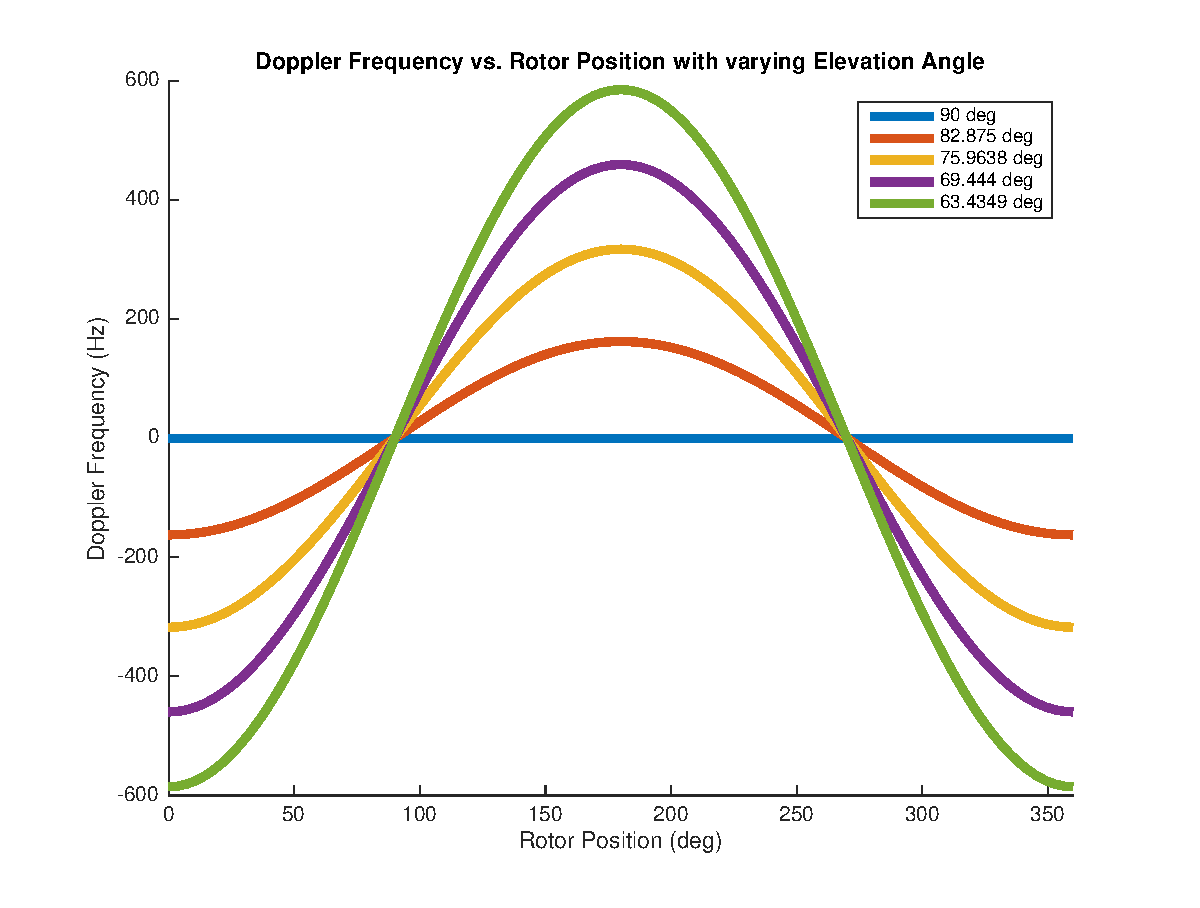
\includegraphics[width=10cm]{images/background/2d_theoretical_doppler_profile.eps}
		\caption{Doppler Frequency vs. Rotor Position with varying Elevation Angle}
		\label{fig:2D_theoretical_doppler}
	\end{center}
\end{figure}

Figure \ref{fig:2D_theoretical_doppler} shows the varying doppler frequency caused by the RBM at various elevation angles of the transmitter. The results of this is a sinusoidal doppler profile in which its amplitude increases as the elevation angle decreases. 

%validation consideration
Since this model has the receiver located at the axis of rotation this model can be seen as a special case of the next 3D models, this is because it is symmetric around the axis of rotation. Therefore any placement of the transmitter in 3D space can be distilled down to a 2D profile as such. This symmetry should then be mirrored in the ray tracing simulation as verification.

\subsection{3D Geometric Model}
The three dimensional geometric model is categorized by the position of the rotor blade and the position of the signal source. Since the rotor blade has a specific airfoil shape the models will take that into account through an approximation of that surface. The first model will be representative of having the transmitter inline with both the receiver and the blade, with the transmitter in both fore and aft positions. The next model will have the rotor approaching both the receiver and transmitter, and lastly the rotor will be receding from both the receiver and transmitter. All of the 3D models will have the receiver positioned offset from the axis of rotation.

\subsubsection{Transmitter inline with Receiver and Rotor Blade}
%go over the 3d model for the tx inline with blade fore and aft
The first two models as mentioned above fall under the criteria of the transmitter being inline with both the rotor blade and the offset receiver. 

Figure \ref{fig:3D_model_90az} depicts the transmitter at a 90\textdegree \space azimuth angle, which places it inline with the position of the receiver and the current location of the rotating blades. 

%describe the situation and the position of the objects
The objects in \ref{fig:3D_model_90az}  are similar to the ones previously stated in the 2D case. The X and Y axis are specifically drawn in blue and red respectfully, with the Z axis now the green dashed line and altitude is now denoted with a measurement bar. The receiver offset in the +Y direction is now stated. and the Blades are now colored gray. All other variables and colors denote their objects as previously stated in the 2D case. 

%3d pictures
\begin{figure}
	\begin{center}
		\includegraphics[width=15cm]{images/background/3d_geometry_tx_90az.eps}
		\caption{3D Geometric model with Tx at Azimuth angle of 90\textdegree}
		\label{fig:3D_model_90az}
	\end{center}
\end{figure}

%formulate the geometric equations
(equations doppler profile 90 deg)

%doppler profile result
\begin{figure}
	\begin{center}
		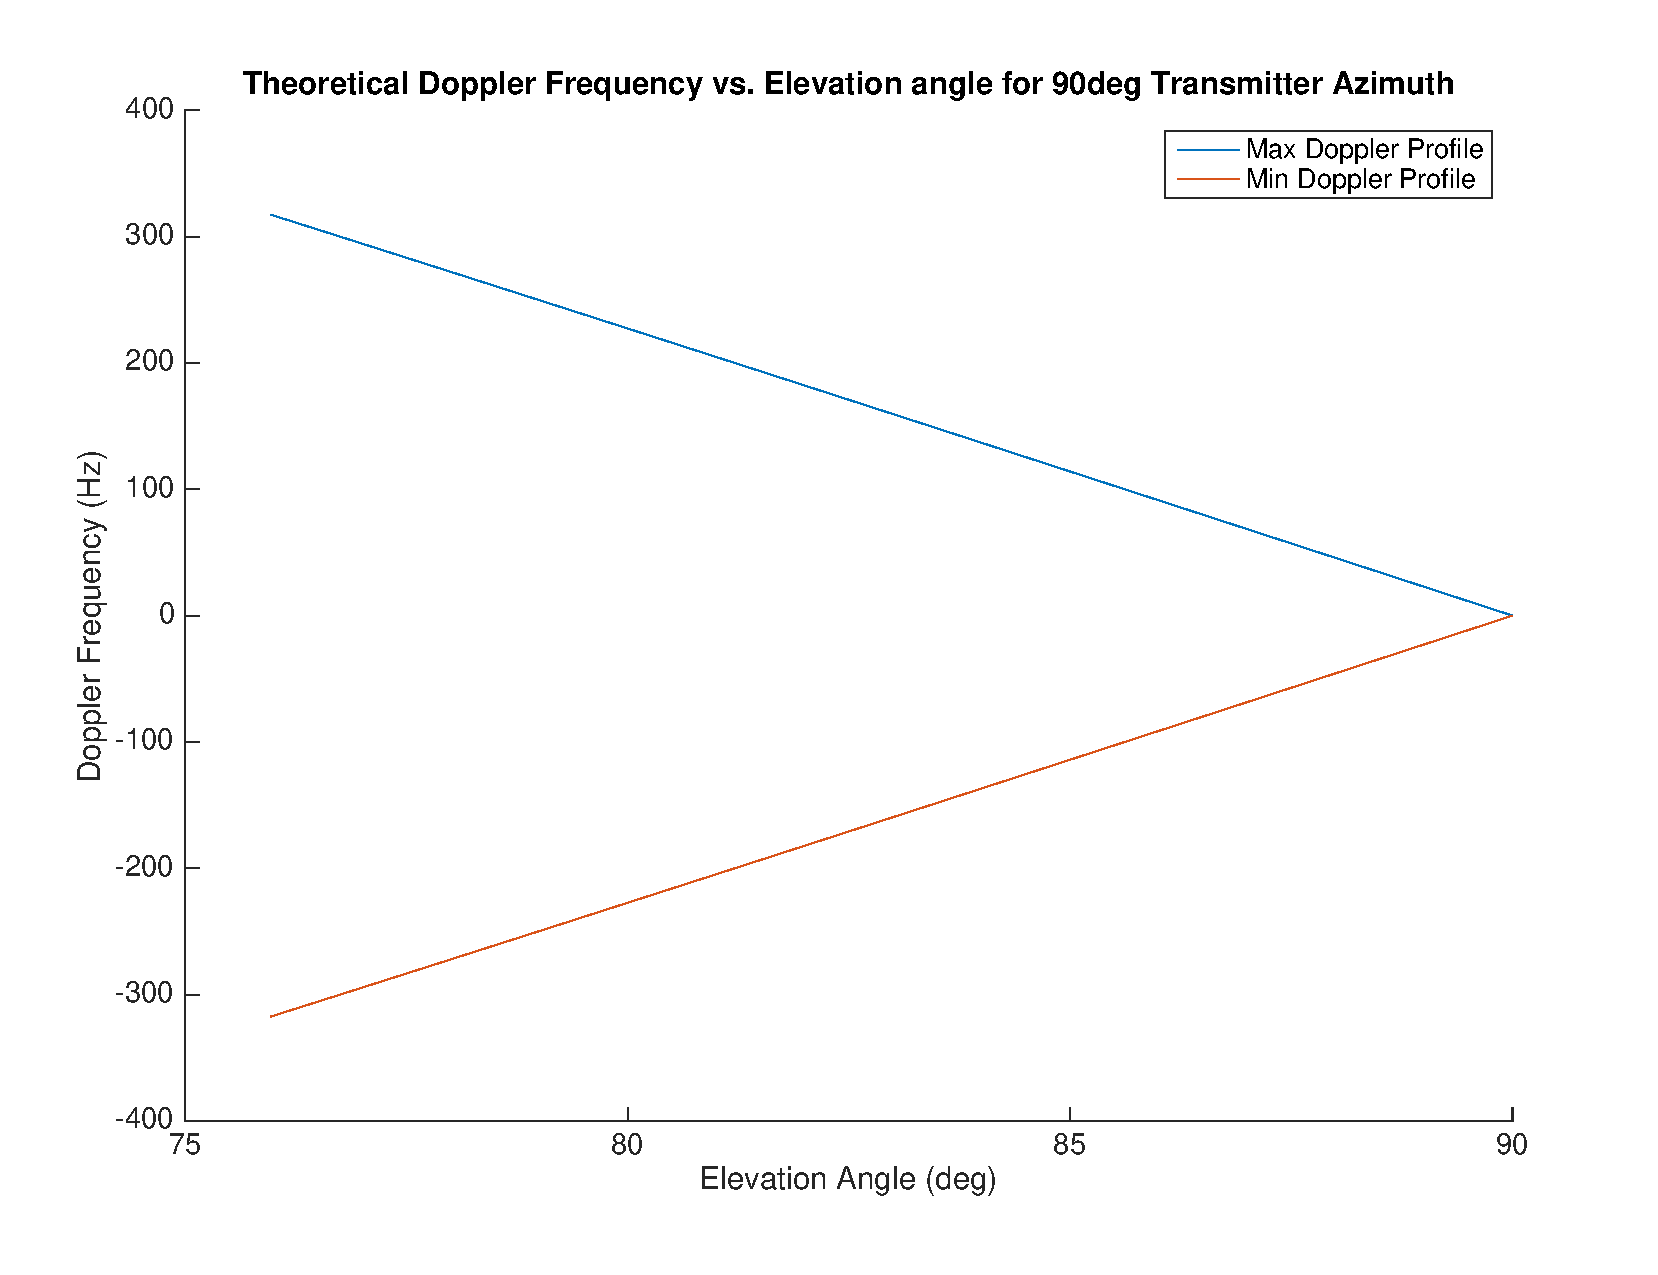
\includegraphics[width=10cm]{images/background/3d_geometry_tx_90az_doppler_profile.eps}
		\caption{Doppler profile of Tx at Azimuth angle of 90\textdegree}
		\label{fig:3D_model_90az_doppler}
	\end{center}
\end{figure}

Figure \ref{fig:3D_model_90az_doppler} shows the maximum and minimum doppler values versus elevation angle for a transmitter at an azimuth angle of 90\textdegree. The elevation angle is limited by the reflection angle, caused by the limited distance between the tip of the blade and the location of the receiver. This limitation constrains the doppler profile causing inaccurate transmitter elevation estimation at this transmitter azimuth position.

Figure \ref{fig:3D_model_270az} depicts the transmitter at a 270\textdegree \space azimuth angle, which places it inline with the position of the receiver and the current location of the rotating blades. This placement of the transmitter behind the helicopter is different from the situation in figure \ref{fig:3D_model_90az} because the value of $\theta_r$ is now not limited by the tip of the rotor and can go to smaller elevation angles.

\begin{figure}
	\begin{center}
		\includegraphics[width=15cm]{images/background/3d_geometry_tx_270az.eps}
		\caption{3D Geometric model with Tx at Azimuth angle of 270\textdegree}
		\label{fig:3D_model_270az}
	\end{center}
\end{figure}

%formulate the geometric equations
(equations doppler profile 270 deg)

%doppler profile result
\begin{figure}
	\begin{center}
		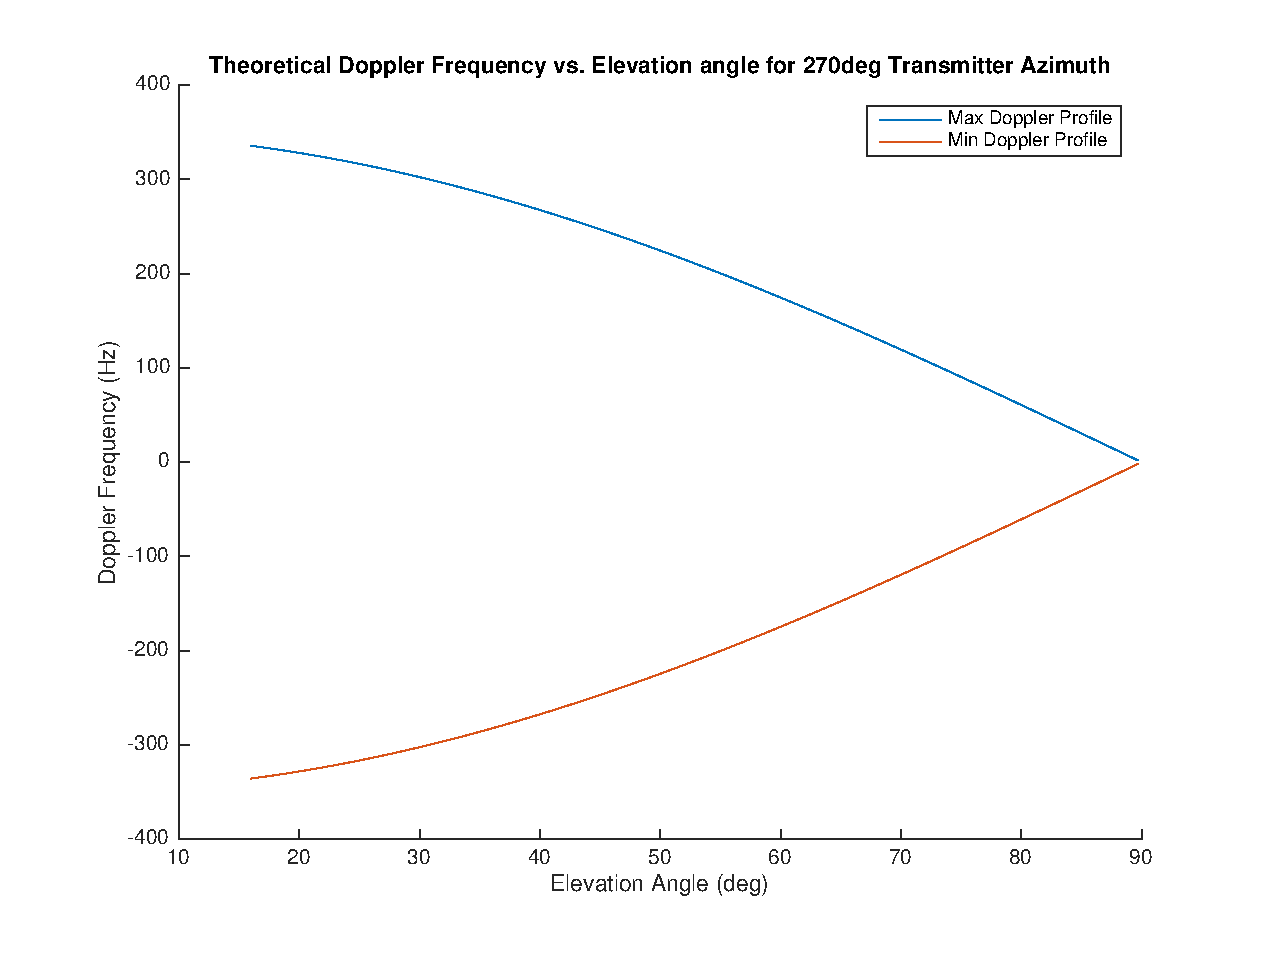
\includegraphics[width=10cm]{images/background/3d_geometry_tx_270az_doppler_profile.eps}
		\caption{Doppler profile of Tx at Azimuth angle of 270\textdegree}
		\label{fig:3D_model_270az_doppler}
	\end{center}
\end{figure}

Figure \ref{fig:3D_model_270az_doppler} shows the maximum and minimum doppler values versus elevation angle for a transmitter at an azimuth angle of 270\textdegree. The data from the figure is similar to the data from the previous figure \ref{fig:3D_model_90az} but does not exhibit the limitation on the reflection angle, allowing for smaller elevation angles and larger doppler shifts to occur.

\subsubsection{Approaching Model}
%go over the 3d model for the approaching blade
The approaching model shown in figure \ref{fig:3D_model_180az} depicts the transmitter at an azimuth of 180 \textdegree \space and the axis of X has now been rotated to be -X. The direction of the rotor blades is depicted ,in green, to follow the previous assumptions.

%describe the situation and the position of the objects
This case of the 3D model places the transmitter at 180 \textdegree \space so that the oncoming blades move toward both the receiver and the transmitter at the same time. This particular placement will cause a positive doppler profile because the blades will be moving in the direction of both objects, compressing the reflected wave accordingly.

%3d picture
\begin{figure}
	\begin{center}
		\includegraphics[width=15cm]{images/background/3d_geometry_tx_180az.eps}
		\caption{3D Geometric model with Tx at Azimuth angle of 180\textdegree}
		\label{fig:3D_model_180az}
	\end{center}
\end{figure}

%formulate the geometric equations
(equations doppler profile 180 deg)

%doppler profile result
\begin{figure}
	\begin{center}
		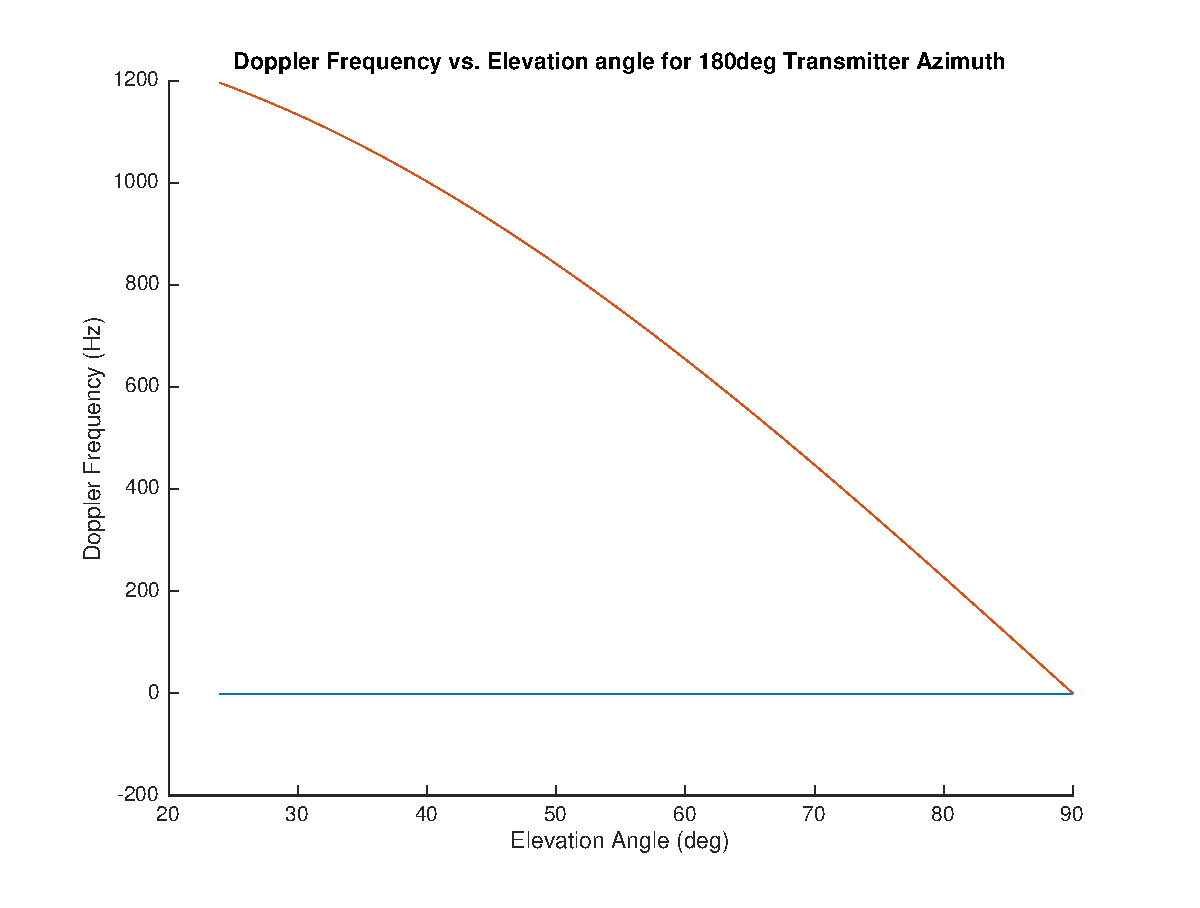
\includegraphics[width=10cm]{images/background/3d_geometry_tx_180az_doppler_profile.eps}
		\caption{Doppler profile of Tx at Azimuth angle of 180\textdegree}
		\label{fig:3D_model_180az_doppler}
	\end{center}
\end{figure}

Figure \ref{fig:3D_model_180az_doppler} shows the maximum and minimum doppler values versus elevation angle for a transmitter at an azimuth angle of 180\textdegree. The data from the figure shows the maximum of the doppler profile decrease as the elevation angle gets larger.

\subsubsection{Receding Model}
%go over the 3d model for the receding blade
The receding model shown in figure \ref{fig:3D_model_0az} depicts the transmitter at an azimuth of 0 \textdegree \space where the axis positions back to their original places and the direction of the rotor blade is now depicted in red.

%describe the situation and the position of the objects
This case of the 3D model places the transmitter at 0 \textdegree \space so that the receding blades move away from both the receiver and the transmitter at the same time. This particular placement should provide a negative doppler profile because the blades will be moving in the opposite direction of both objects, stretching the reflected wave accordingly.

%3d picture 
\begin{figure}
	\begin{center}
		\includegraphics[width=15cm]{images/background/3d_geometry_tx_0az.eps}
		\caption{3D Geometric model with Tx at Azimuth angle of 0\textdegree}
		\label{fig:3D_model_0az}
	\end{center}
\end{figure}

%formulate the geometric equations
(equations doppler profile 0 deg)

%doppler profile result
\begin{figure}
	\begin{center}
		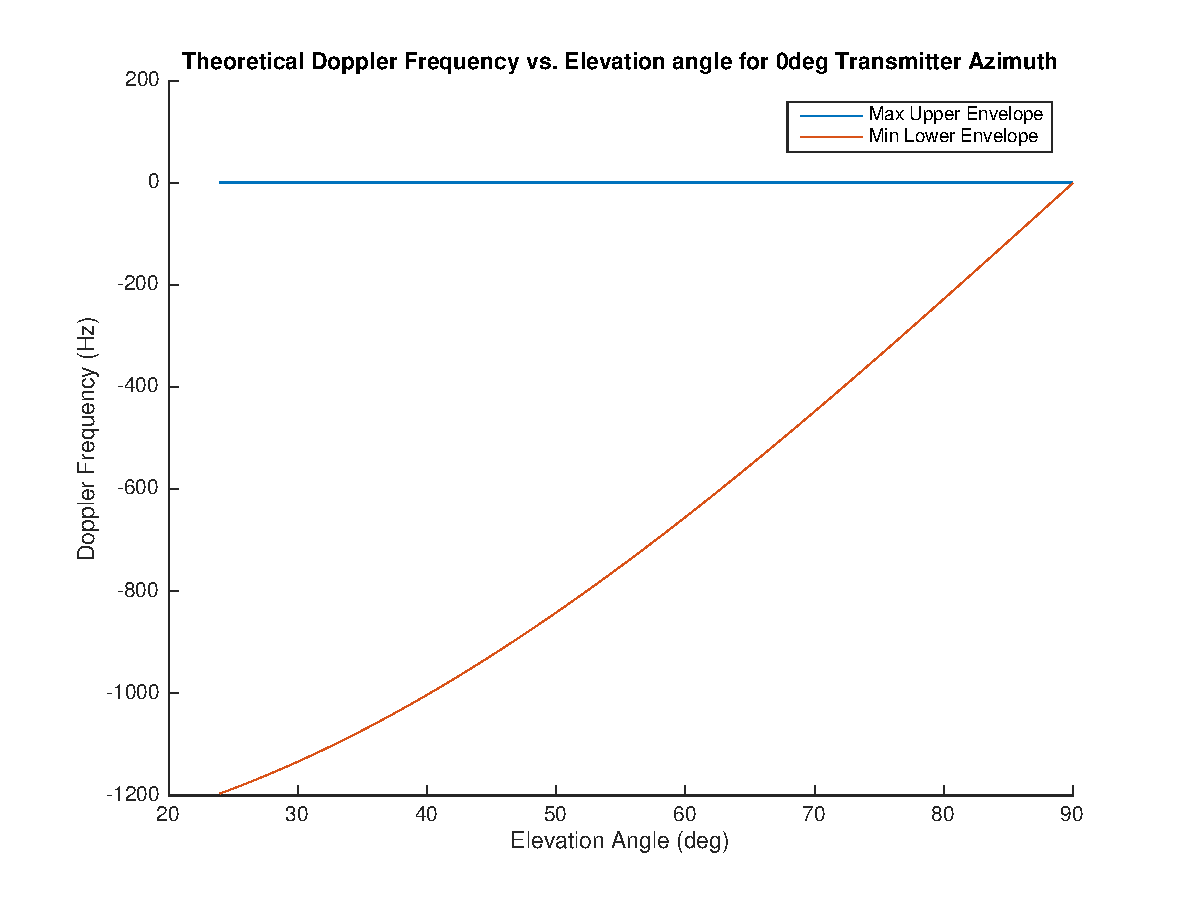
\includegraphics[width=10cm]{images/background/3d_geometry_tx_0az_doppler_profile.eps}
		\caption{Doppler profile of Tx at Azimuth angle of 0\textdegree}
		\label{fig:3D_model_0az_doppler}
	\end{center}
\end{figure}

Figure \ref{fig:3D_model_0az_doppler} shows the maximum and minimum doppler values versus elevation angle for a transmitter at an azimuth angle of 0\textdegree. The data from the figure shows the minimum of the doppler profile increase as the elevation angle gets larger.
